
\section{Liste der anbei NICHT dokumentierten Aufgaben:}
%Die Lösungen können durch das Rückgängig machen der Auskommentierung eingefügt werden. Sie müssen einfach im selben Ordner wie die Aufgabenstellung sein. 
\begin{itemize}
	\item Prakti 1: A5, A6, A7
	\item Prakti 2: A1, A2, A3, A4
	\item Prakti 3: A1, A2, A3, A4
	\item Prakti 4: A1, A2, A3, A4, A5
	\item Prakti 7: A3 
	\item Prakti 10: A8
\end{itemize}
%Uebung 1
\setcounter{section}{1}
\setcounter{subsection}{0}
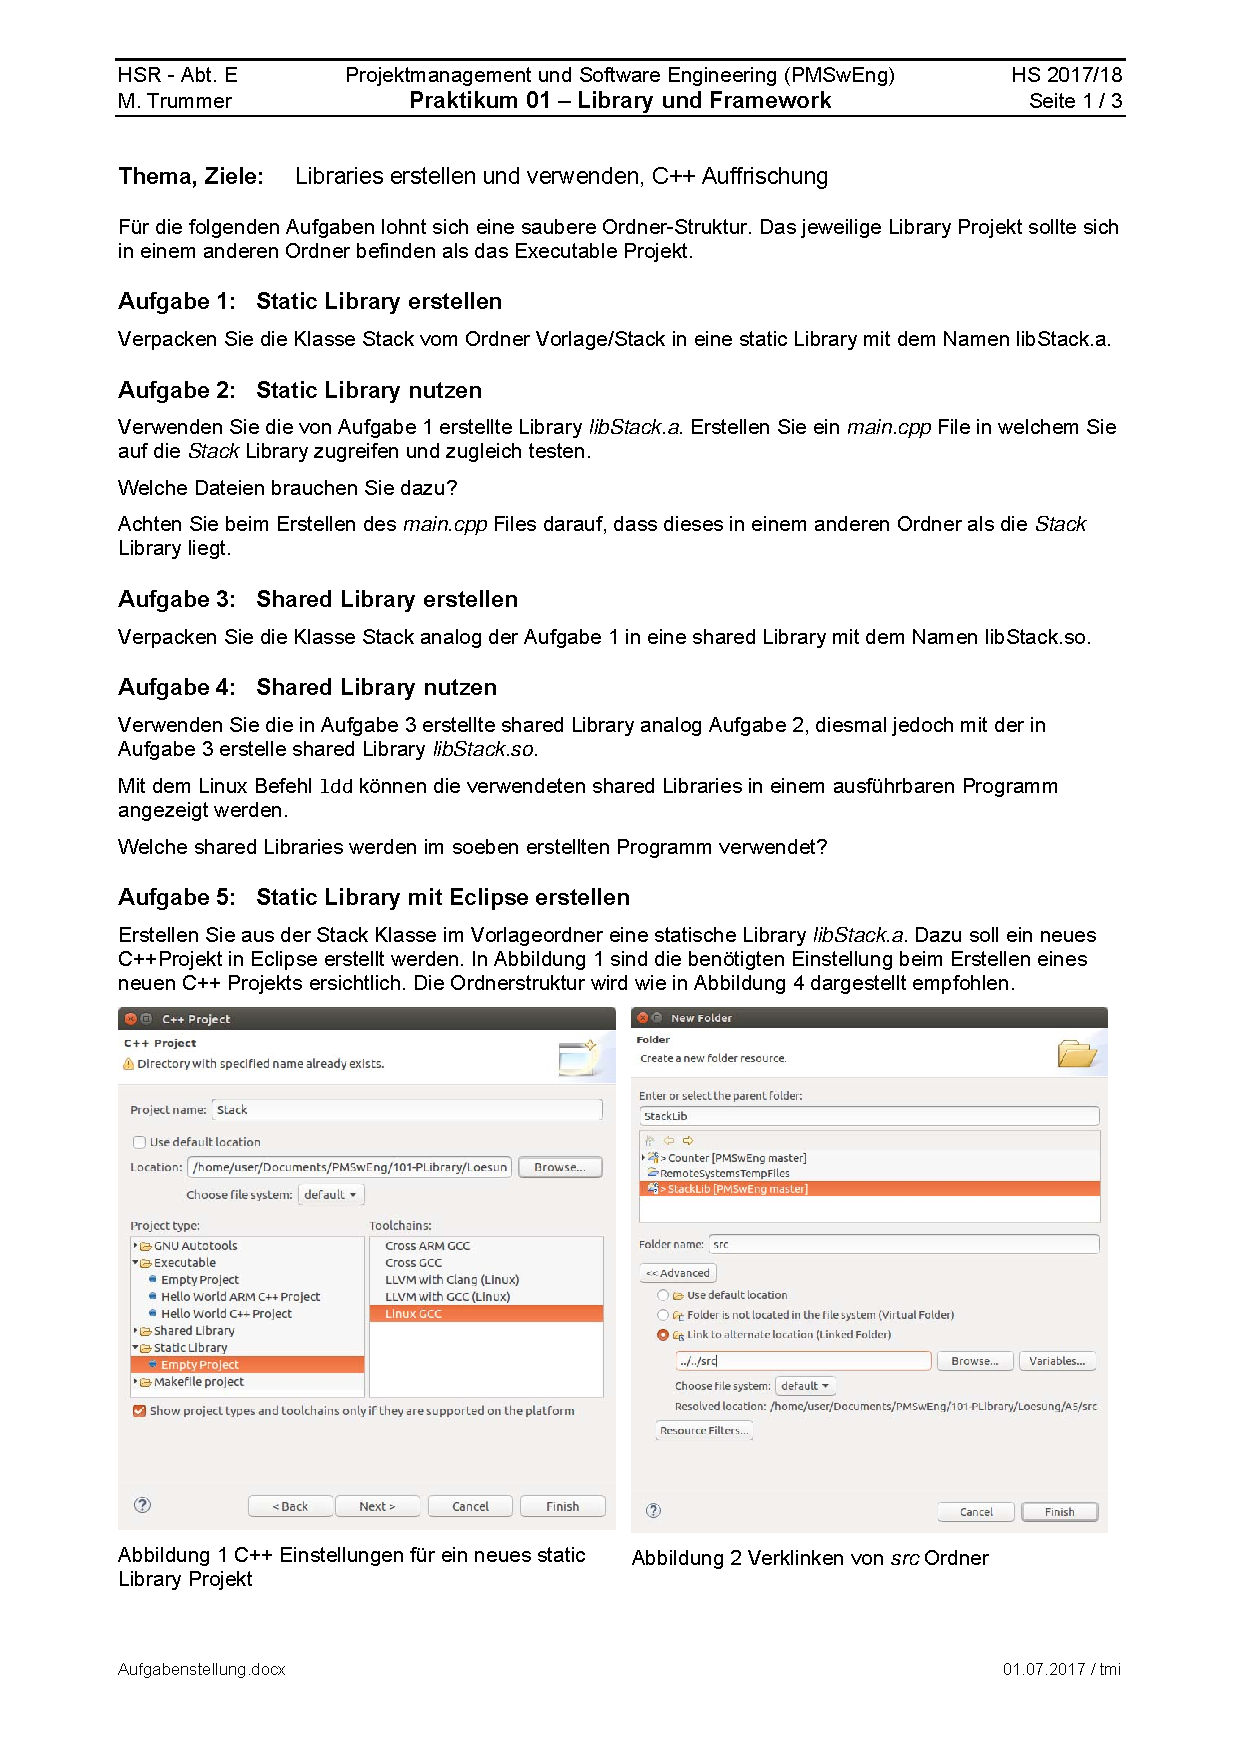
\includepdf[pages=-]{./Uebungen/prak01/Aufgabenstellung.pdf}
%\includepdf[pages=-]{./Uebungen/prak01/Loesung.pdf}
%\subsubsection{A7: Counter.h}
%\lstinputlisting{./Uebungen/prak01/Loesung/A7/src/Counter.h}
%\subsubsection{A7: Counter.cpp}
%\lstinputlisting{./Uebungen/prak01/Loesung/A7/src/Counter.cpp}
%\subsubsection{A7: main.cpp}
%\lstinputlisting{./Uebungen/prak01/Loesung/A7/src/main.cpp}
%
%Uebung 2
\setcounter{section}{2}
\setcounter{subsection}{1}
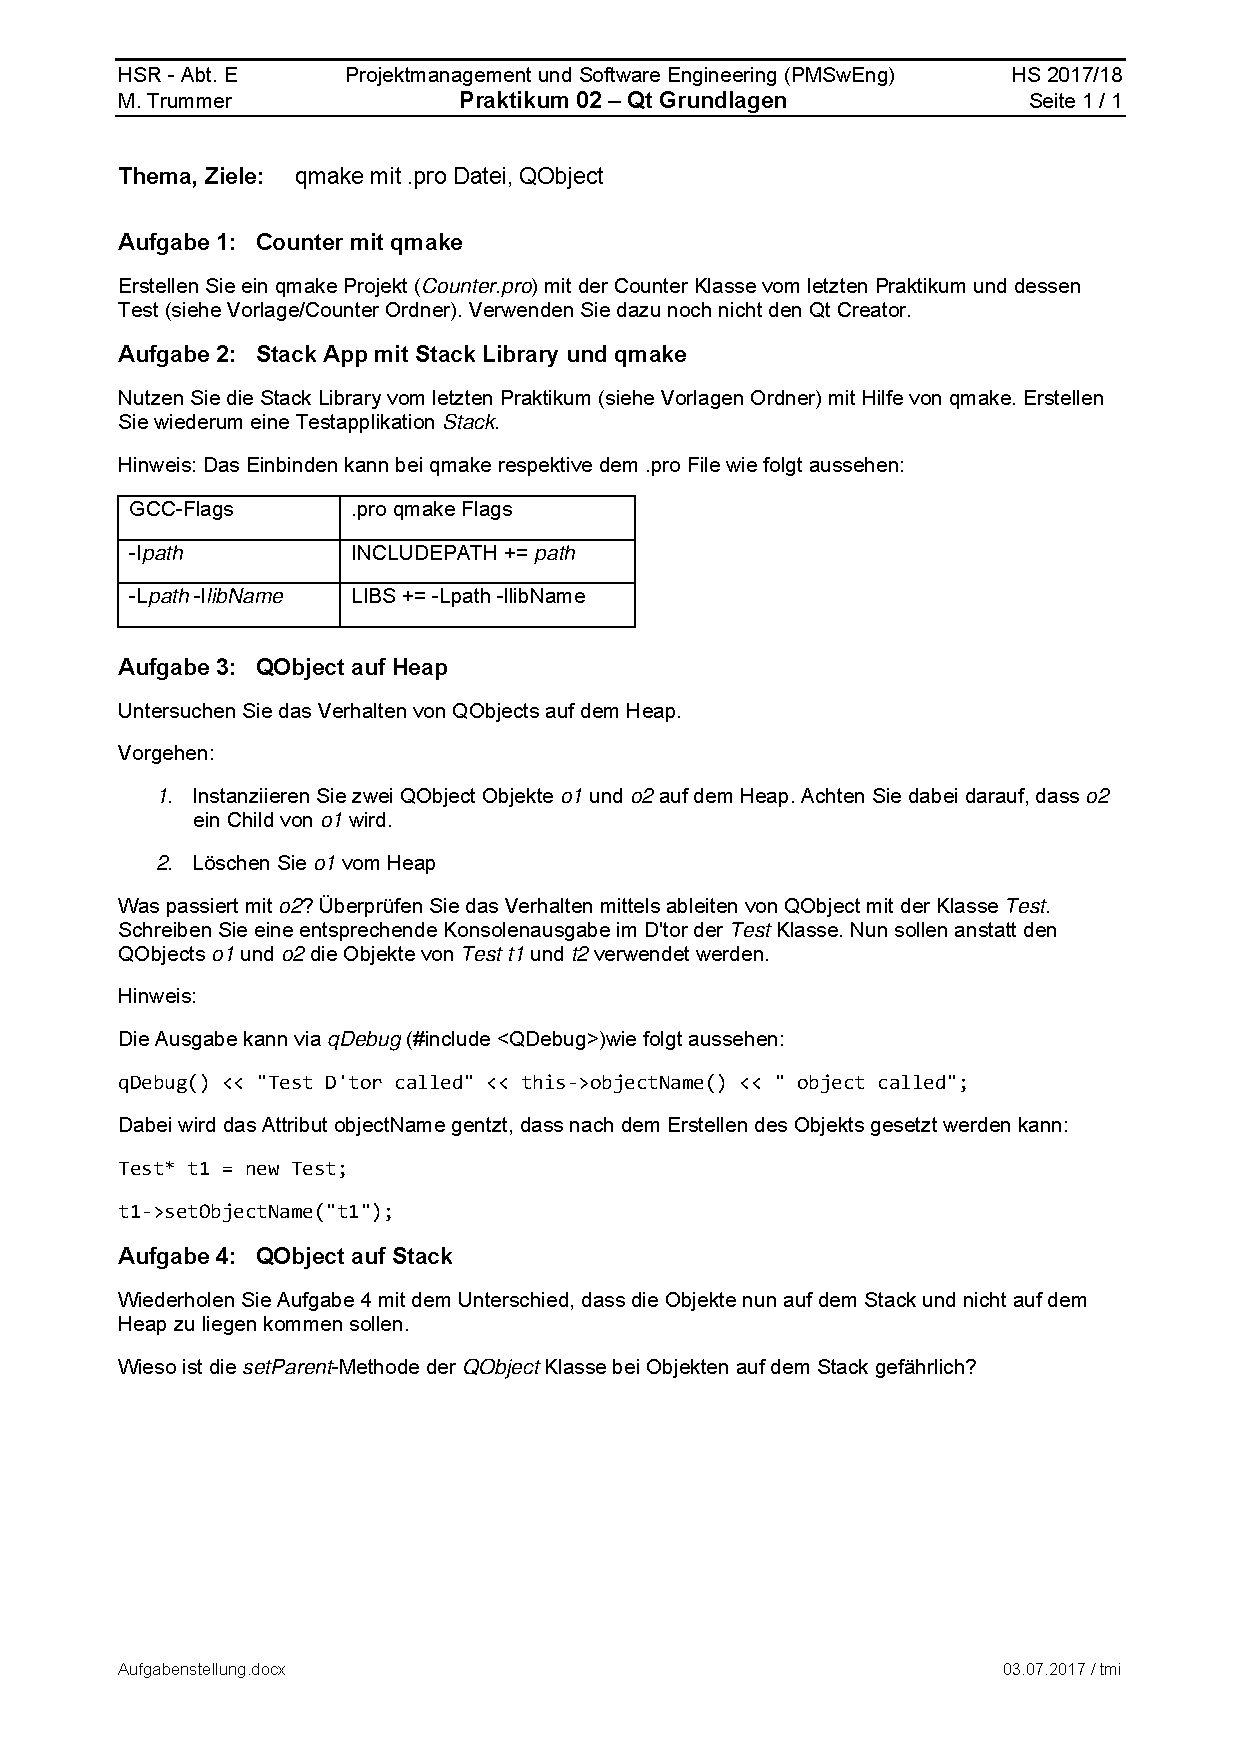
\includepdf[pages=-]{./Uebungen/prak02/Aufgabenstellung.pdf}
%\includepdf[pages=-]{./Uebungen/prak02/Loesung.pdf}
%
%Uebung 3
\setcounter{section}{3}
\setcounter{subsection}{1}
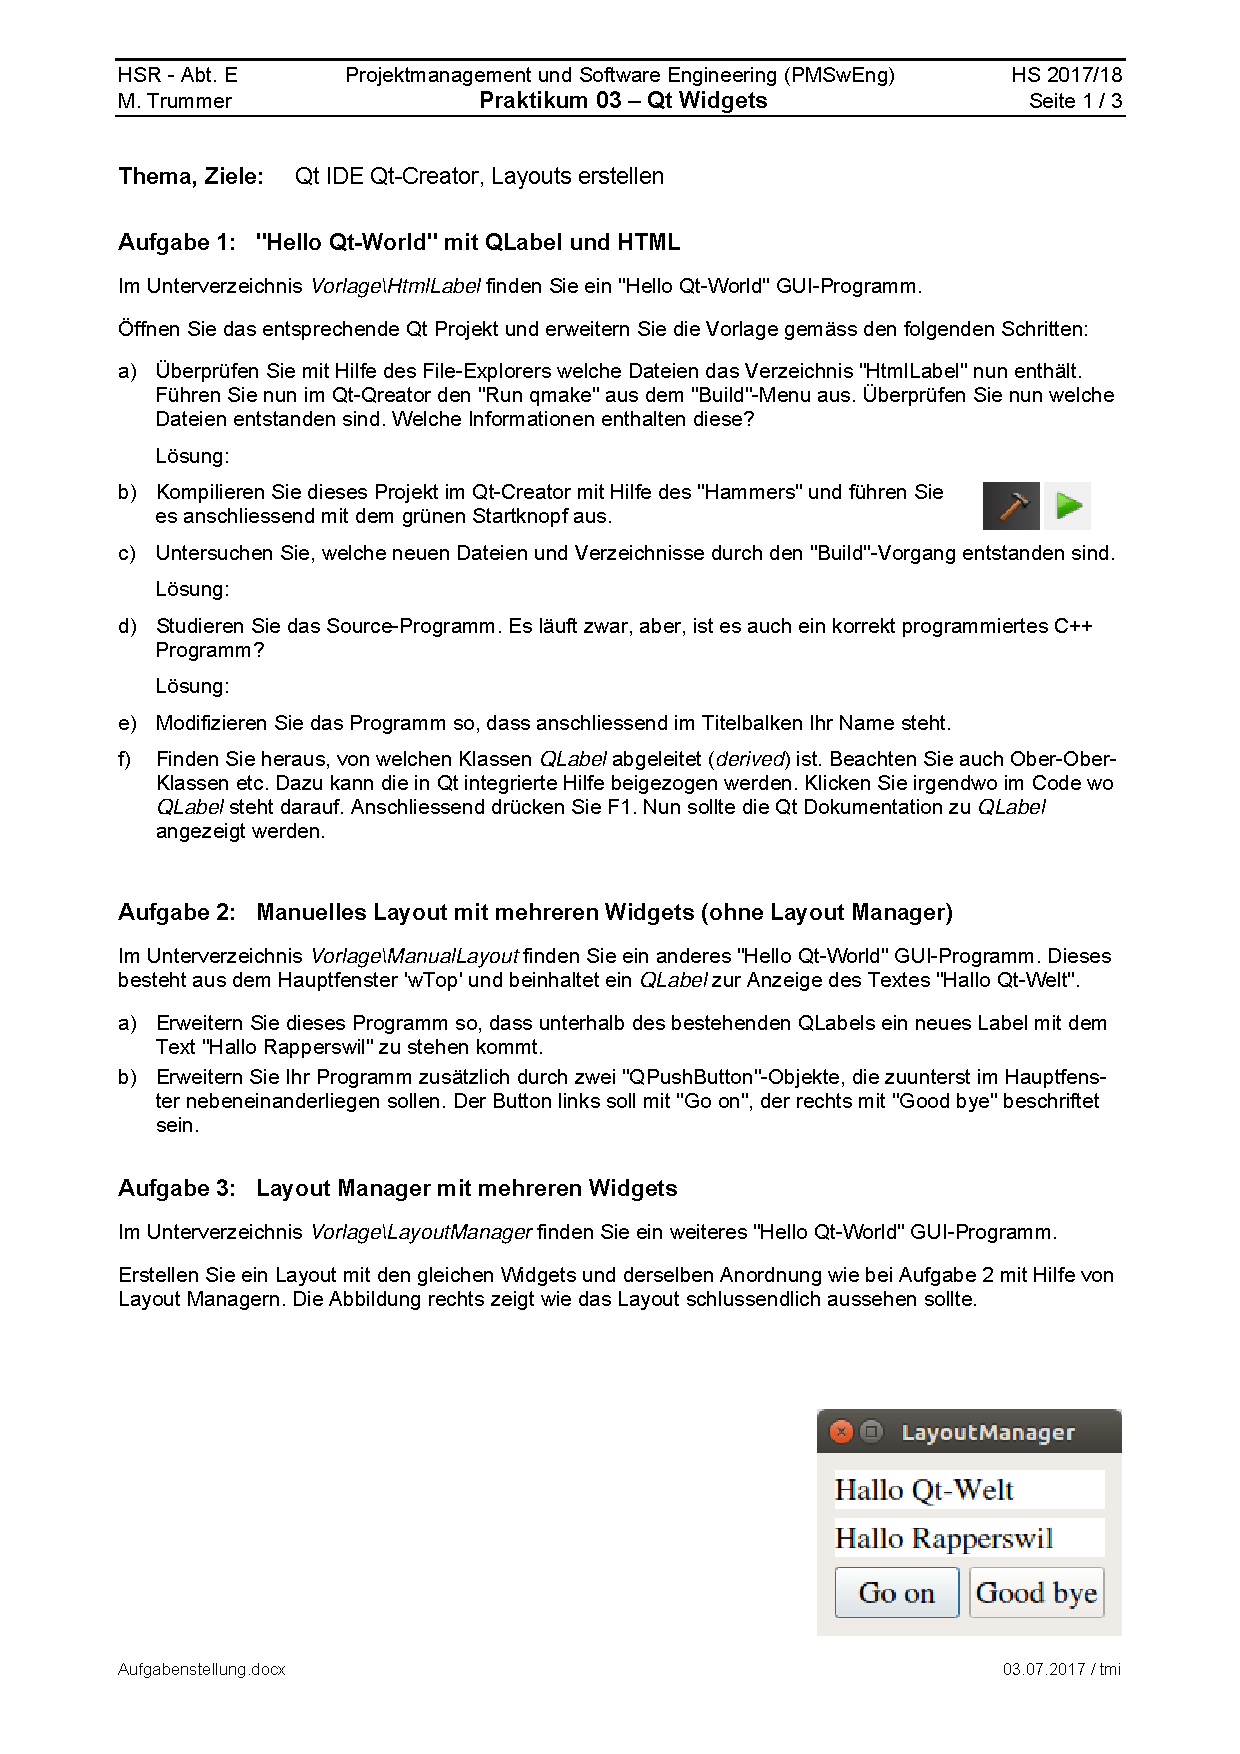
\includepdf[pages=-]{./Uebungen/prak03/Aufgabenstellung.pdf}
%\includepdf[pages=-]{./Uebungen/prak03/Loesung.pdf}

%Uebung 4
\setcounter{section}{4}
\setcounter{subsection}{1}
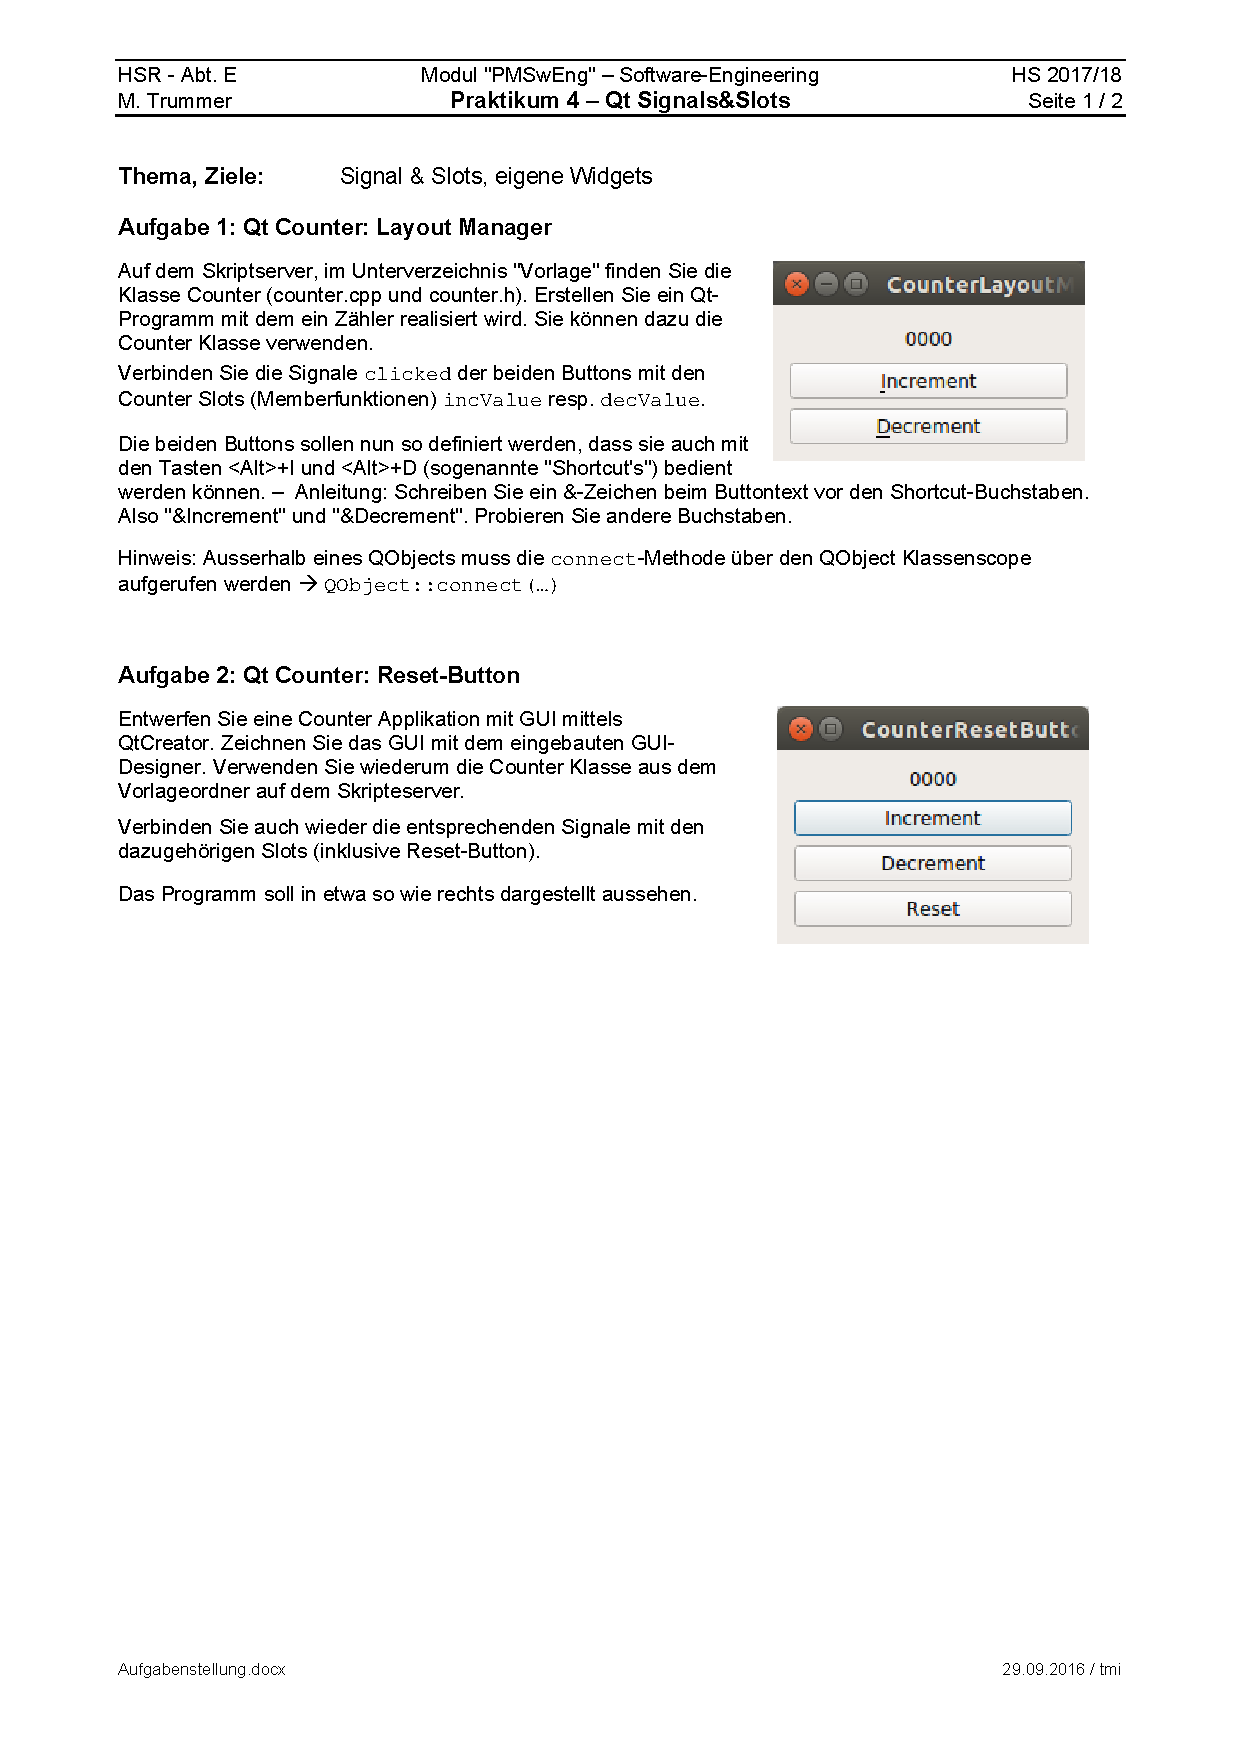
\includepdf[pages=-]{./Uebungen/prak04/Aufgabenstellung.pdf}
%\includepdf[pages=-]{./Uebungen/prak04/Loesung.pdf}
%Uebung 5
\setcounter{section}{5}
\setcounter{subsection}{1}
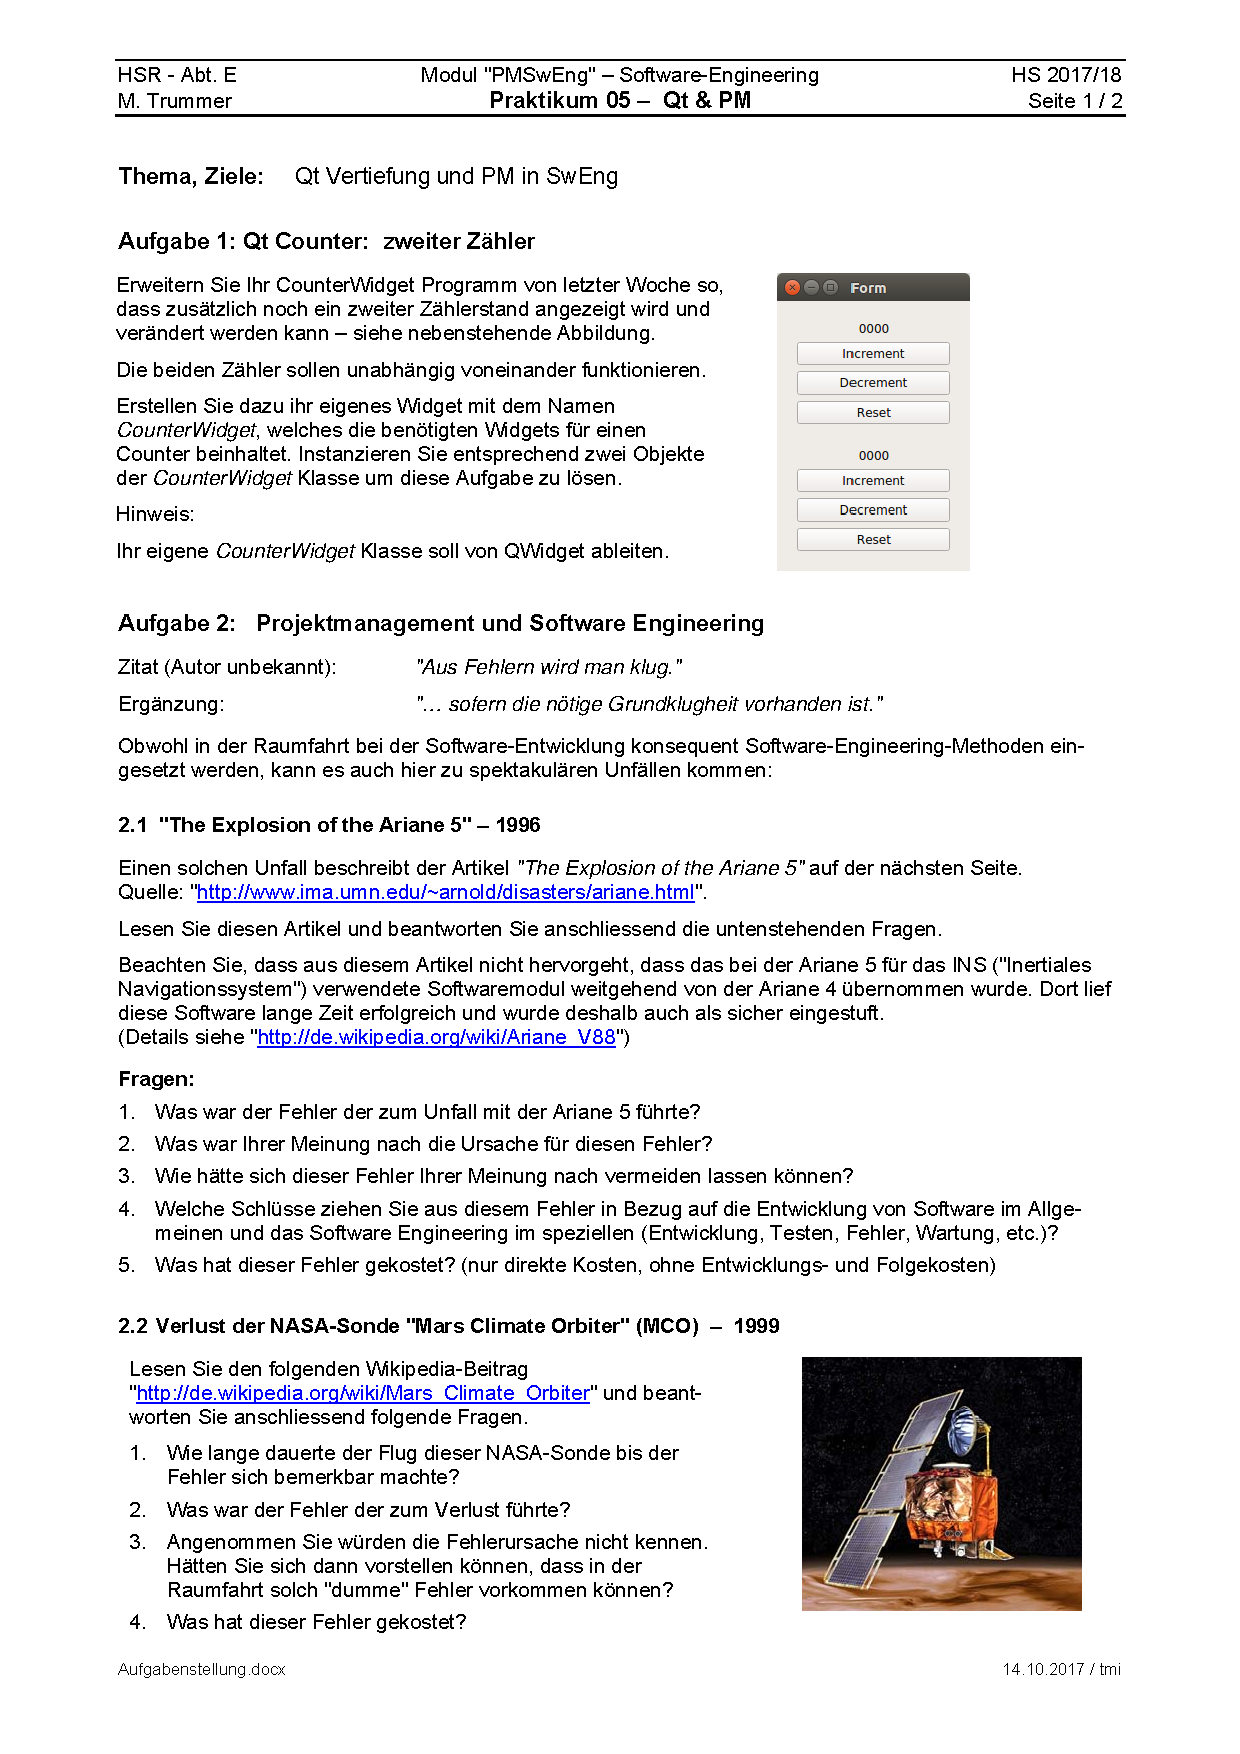
\includepdf[pages=-]{./Uebungen/prak05/Aufgabenstellung.pdf}
%\includepdf[pages=-]{./Uebungen/prak05/Loesung.pdf}

%Uebung 6
\setcounter{section}{6}
\setcounter{subsection}{1}
\includepdf[pages=-]{./Uebungen/prak06/Aufgabenstellung.pdf}
%\includepdf[pages=-]{./Uebungen/prak06/Loesung.pdf}

%Uebung 7
\setcounter{section}{7}
\setcounter{subsection}{1}
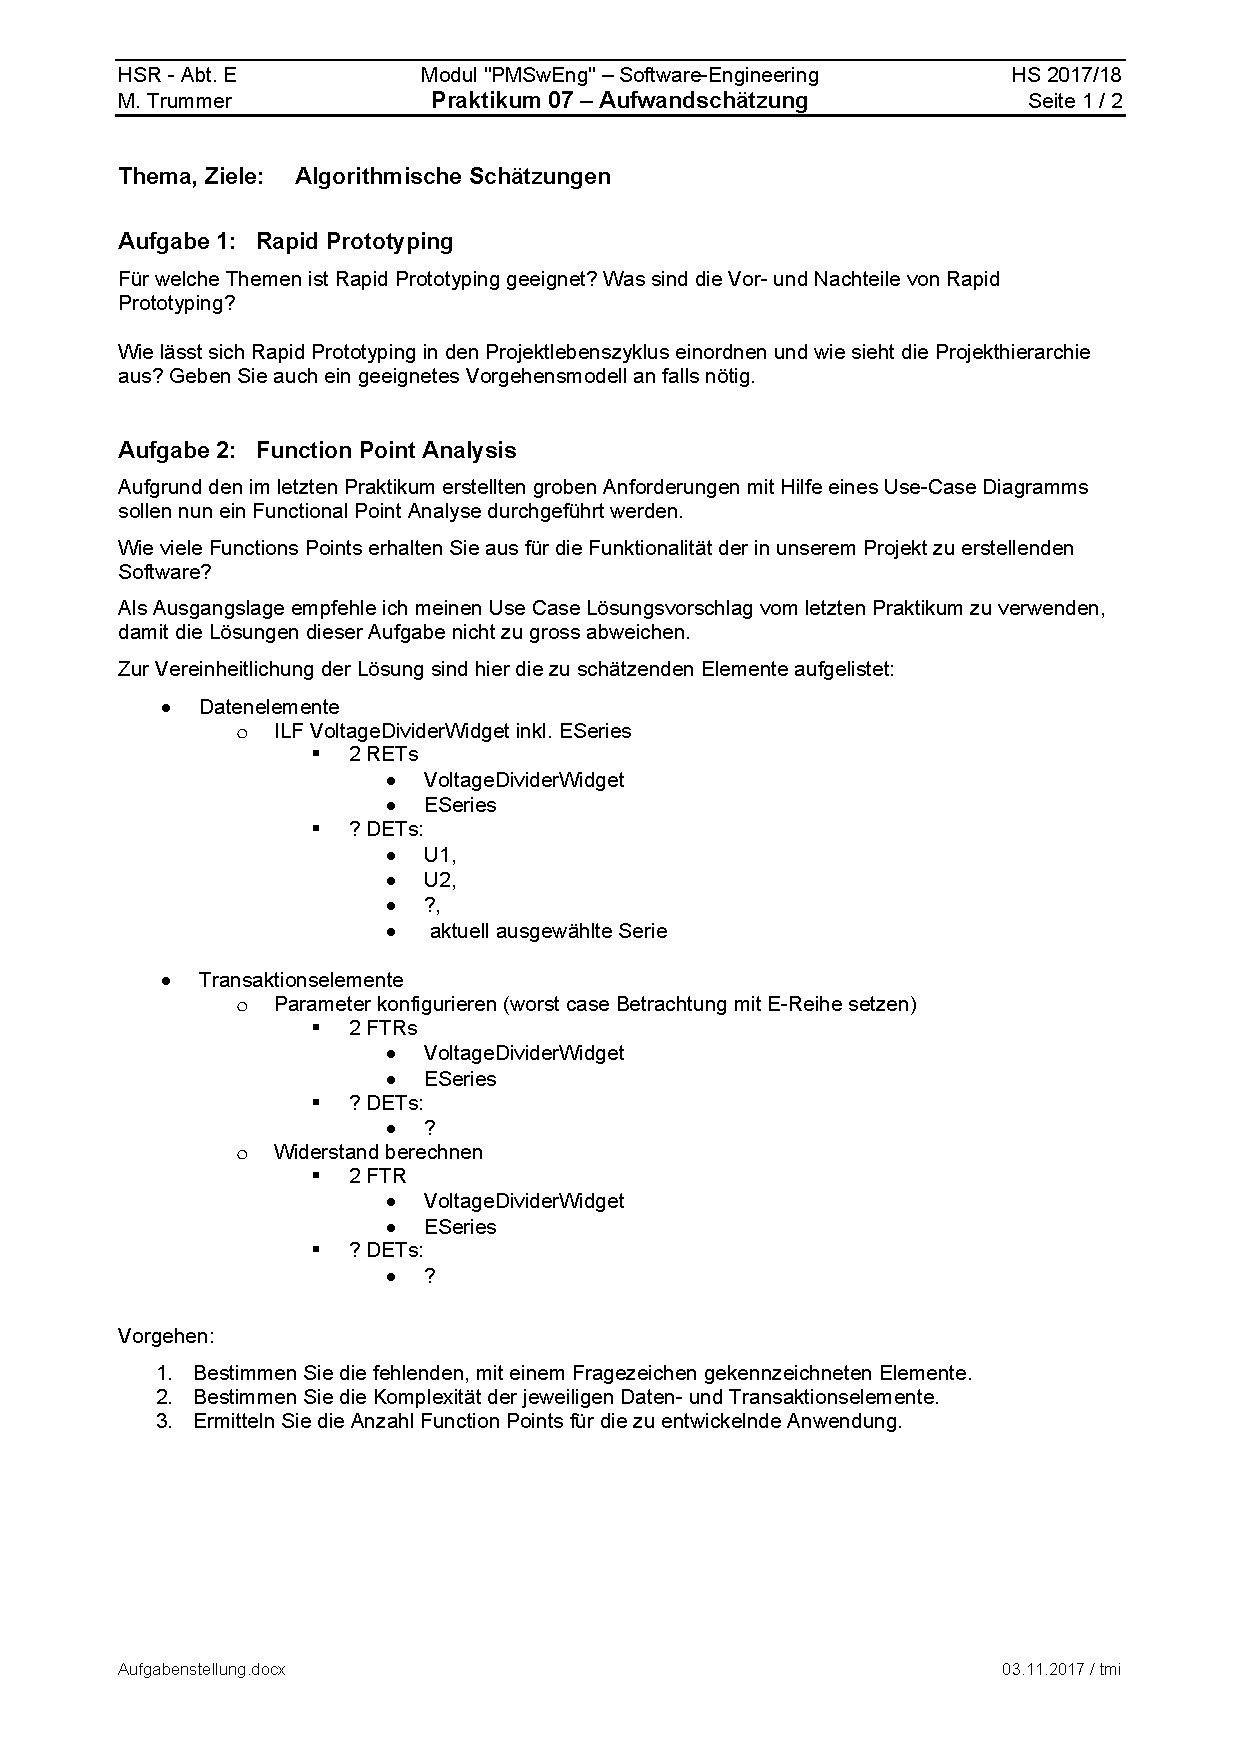
\includepdf[pages=-]{./Uebungen/prak07/Aufgabenstellung.pdf}
%\includepdf[pages=-]{./Uebungen/prak07/Loesung.pdf}
% Übung A3 Einfügen und Dokumentieren

%Uebung 8
\setcounter{section}{8}
\setcounter{subsection}{1}
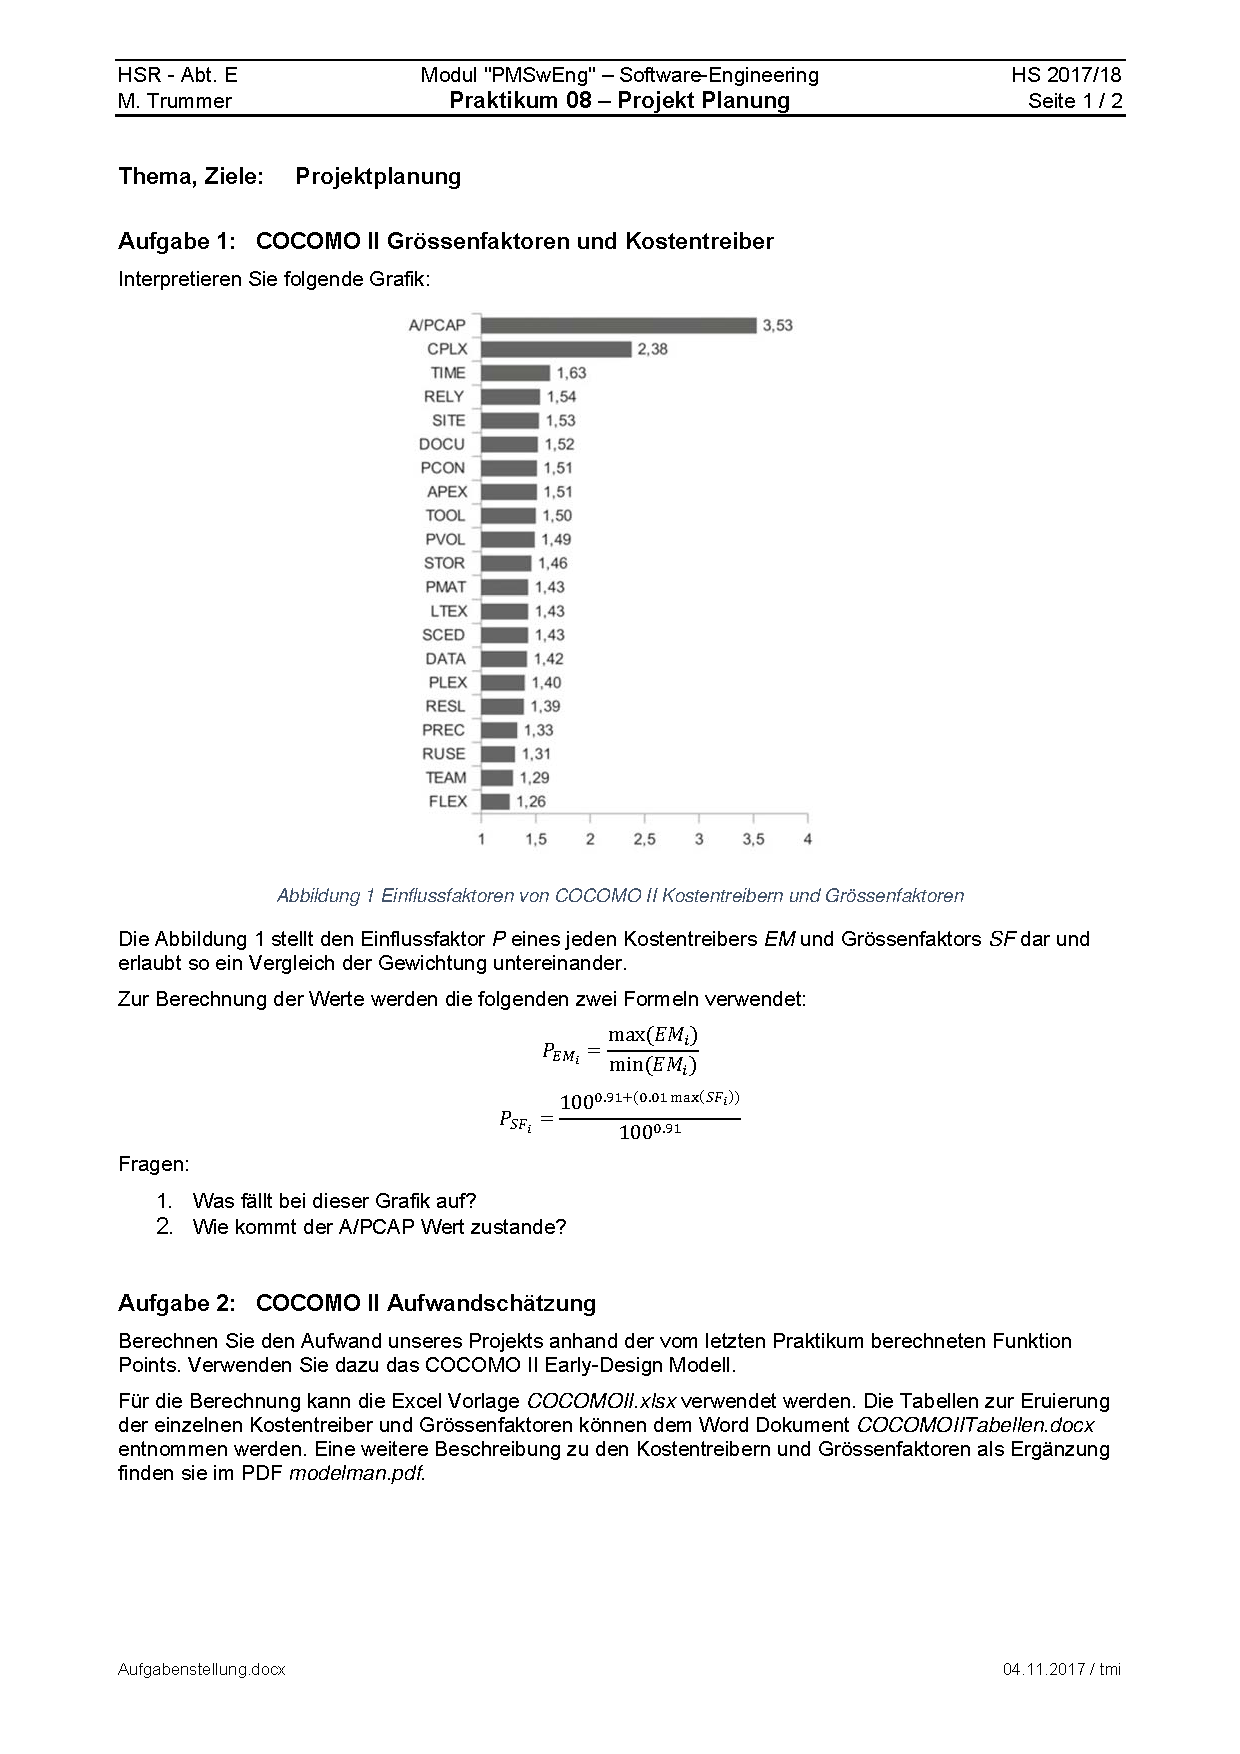
\includepdf[pages=-]{./Uebungen/prak08/Aufgabenstellung.pdf}
%\includepdf[pages=-]{./Uebungen/prak08/Loesung.pdf}
\subsubsection{A2: COCOMO II Tabellen}
%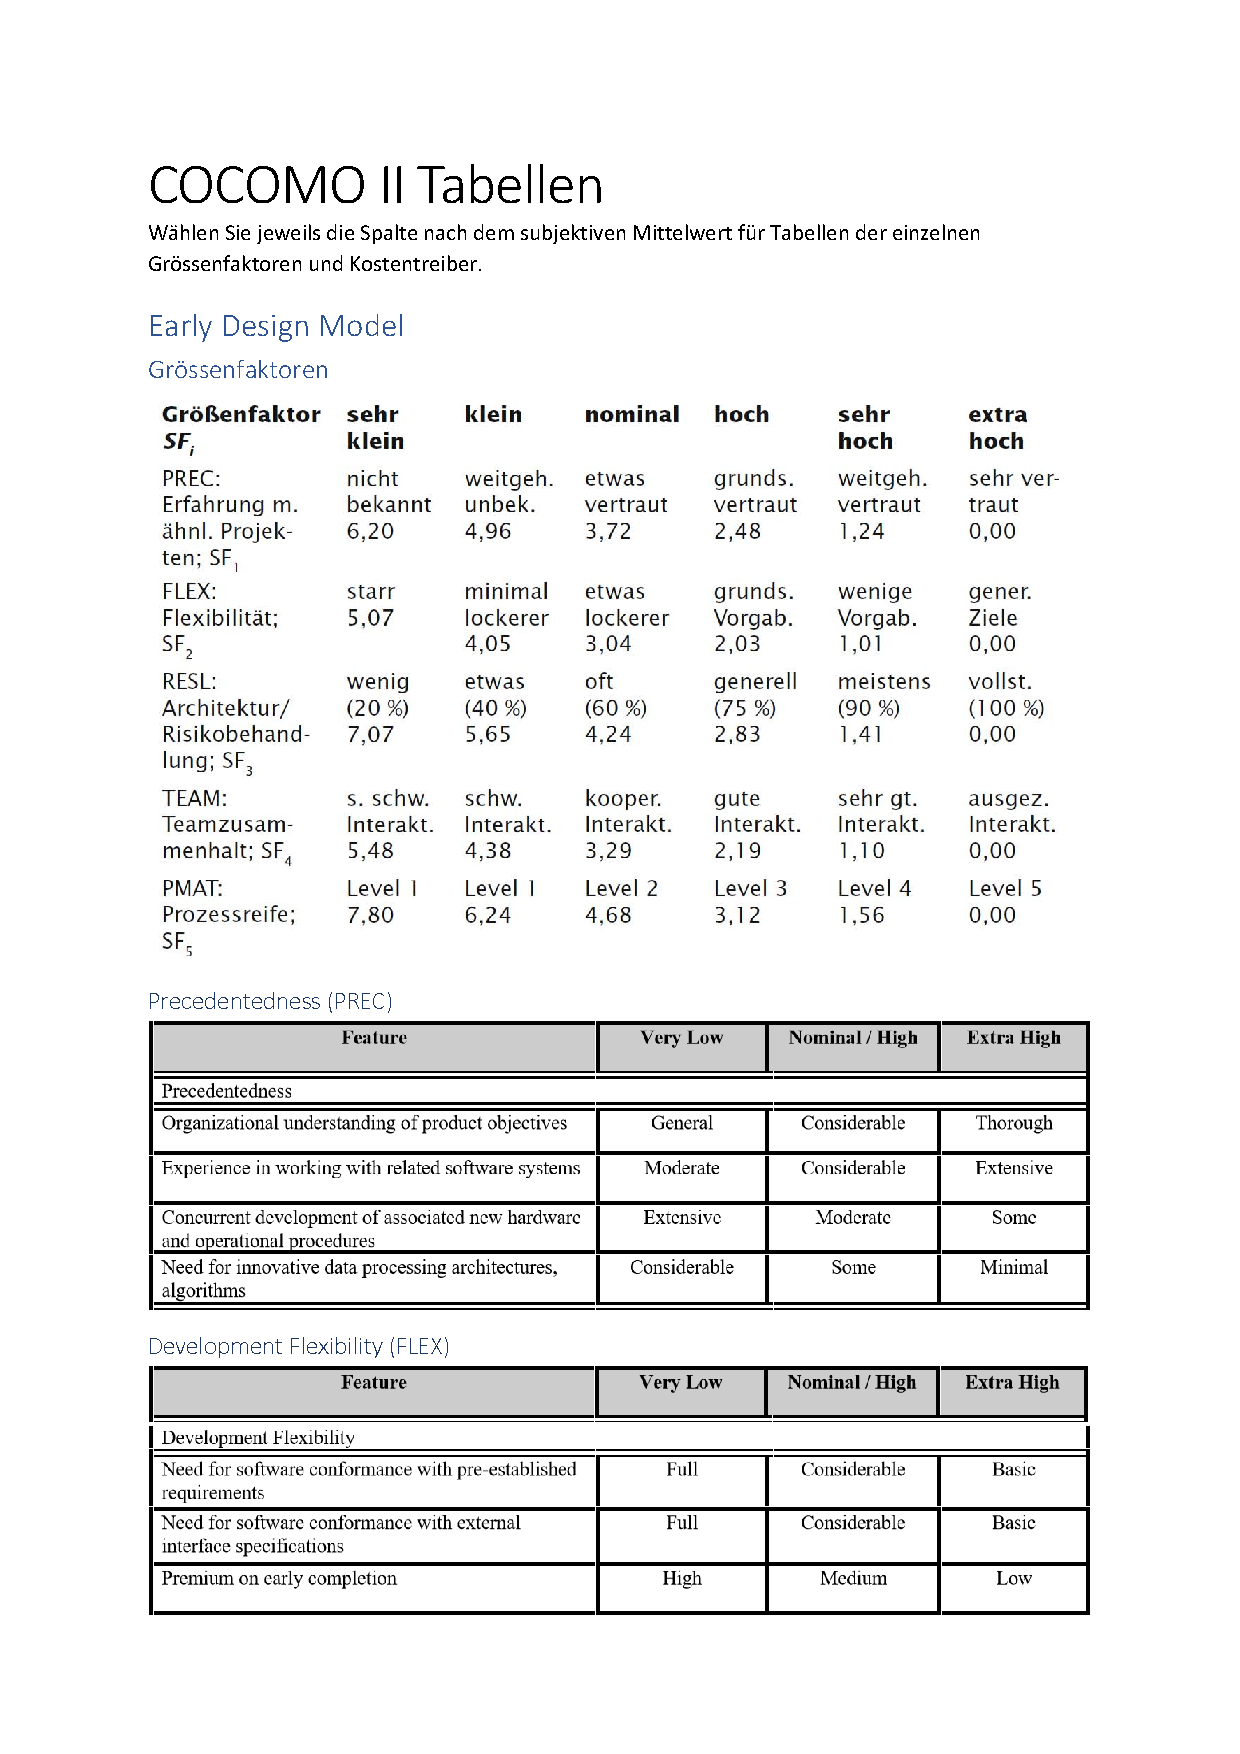
\includepdf[pages=-]{./Uebungen/prak08/Loesung/COCOMOIITabellen.pdf}
%\adjustbox{width=0.9\textwidth}{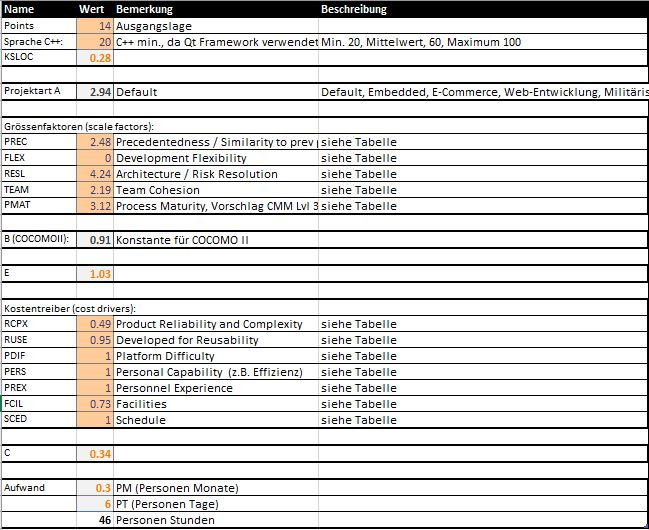
\includegraphics{Figures/COCOMOII}}

%Uebung 9
\setcounter{section}{9}
\setcounter{subsection}{1}

\includepdf[pages=-]{./Uebungen/prak09/Aufgabenstellung.pdf}
%\includepdf[pages=-]{./Uebungen/prak09/Loesung.pdf}

%Uebung 10
\setcounter{section}{10}
\setcounter{subsection}{1}
\includepdf[pages=-]{./Uebungen/prak10/Aufgabenstellung.pdf}
%\includepdf[pages=-]{./Uebungen/prak10/Loesung.pdf}
%\subsubsection{VoltageDividerWidget.cpp}
%\lstinputlisting{./Uebungen/prak10/Loesung/VoltageDivider/src/VoltageDividerWidget.cpp}
%\subsubsection{VoltageDividerWidget.h}
%\lstinputlisting{./Uebungen/prak10/Loesung/VoltageDivider/src/VoltageDividerWidget.h}
%\subsubsection{VoltageDividerWidget.ui}
%\lstinputlisting{./Uebungen/prak10/Loesung/VoltageDivider/src/VoltageDividerWidget.ui}
%\subsubsection{VoltageDivider.cpp}
%\lstinputlisting{./Uebungen/prak10/Loesung/VoltageDivider/src/VoltageDivider.cpp}
%\subsubsection{VoltageDivider.h}
%\lstinputlisting{./Uebungen/prak10/Loesung/VoltageDivider/src/VoltageDivider.h}
%\subsubsection{UserInputValidator.cpp}
%\lstinputlisting{./Uebungen/prak10/Loesung/VoltageDivider/src/UserInputValidator.cpp}
%\subsubsection{UserInputValidator.h}
%\lstinputlisting{./Uebungen/prak10/Loesung/VoltageDivider/src/UserInputValidator.h}

%Uebung 11
\setcounter{section}{11}
\setcounter{subsection}{1}
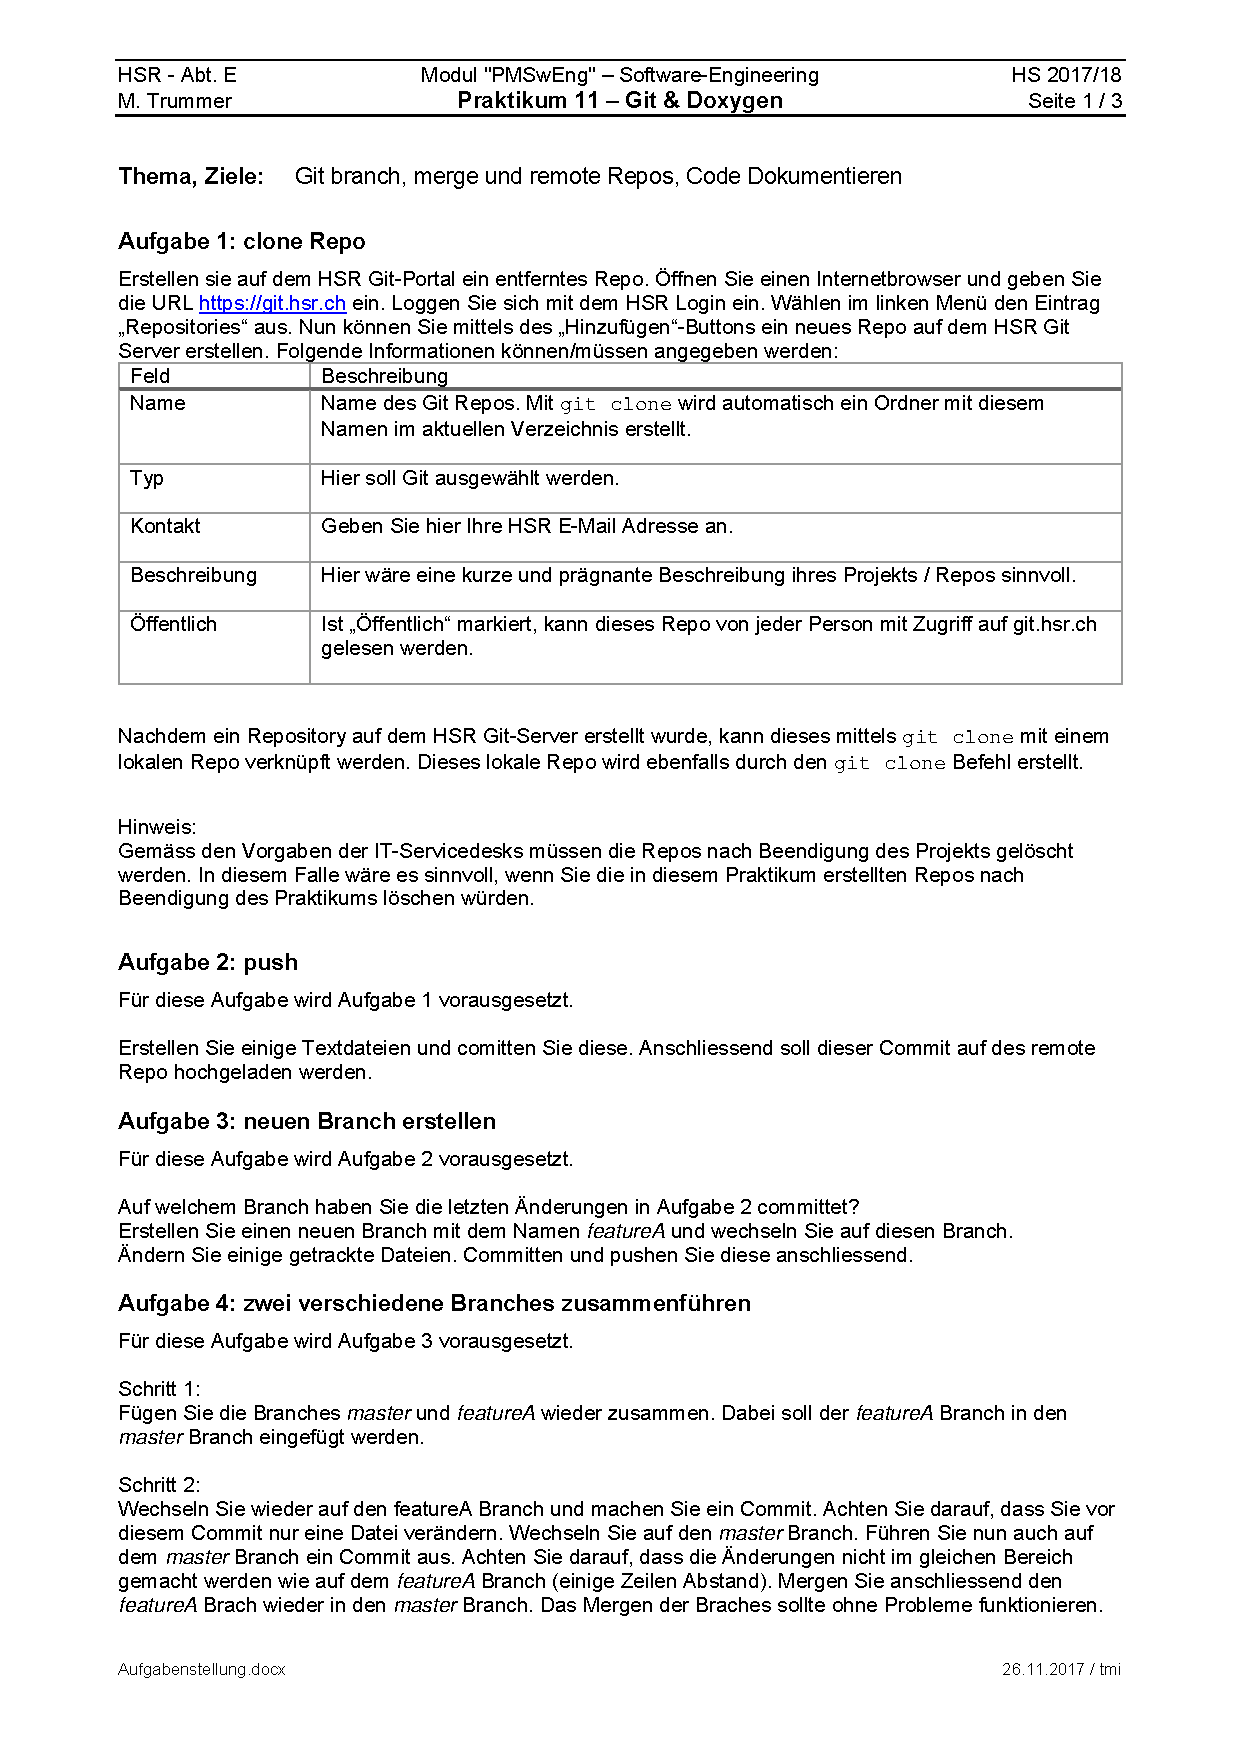
\includepdf[pages=-]{./Uebungen/prak11/Aufgabenstellung.pdf}
%\includepdf[pages=-]{./Uebungen/prak11/Loesung.pdf}

%%Uebung 12
%\setcounter{section}{12}
%\setcounter{subsection}{1}
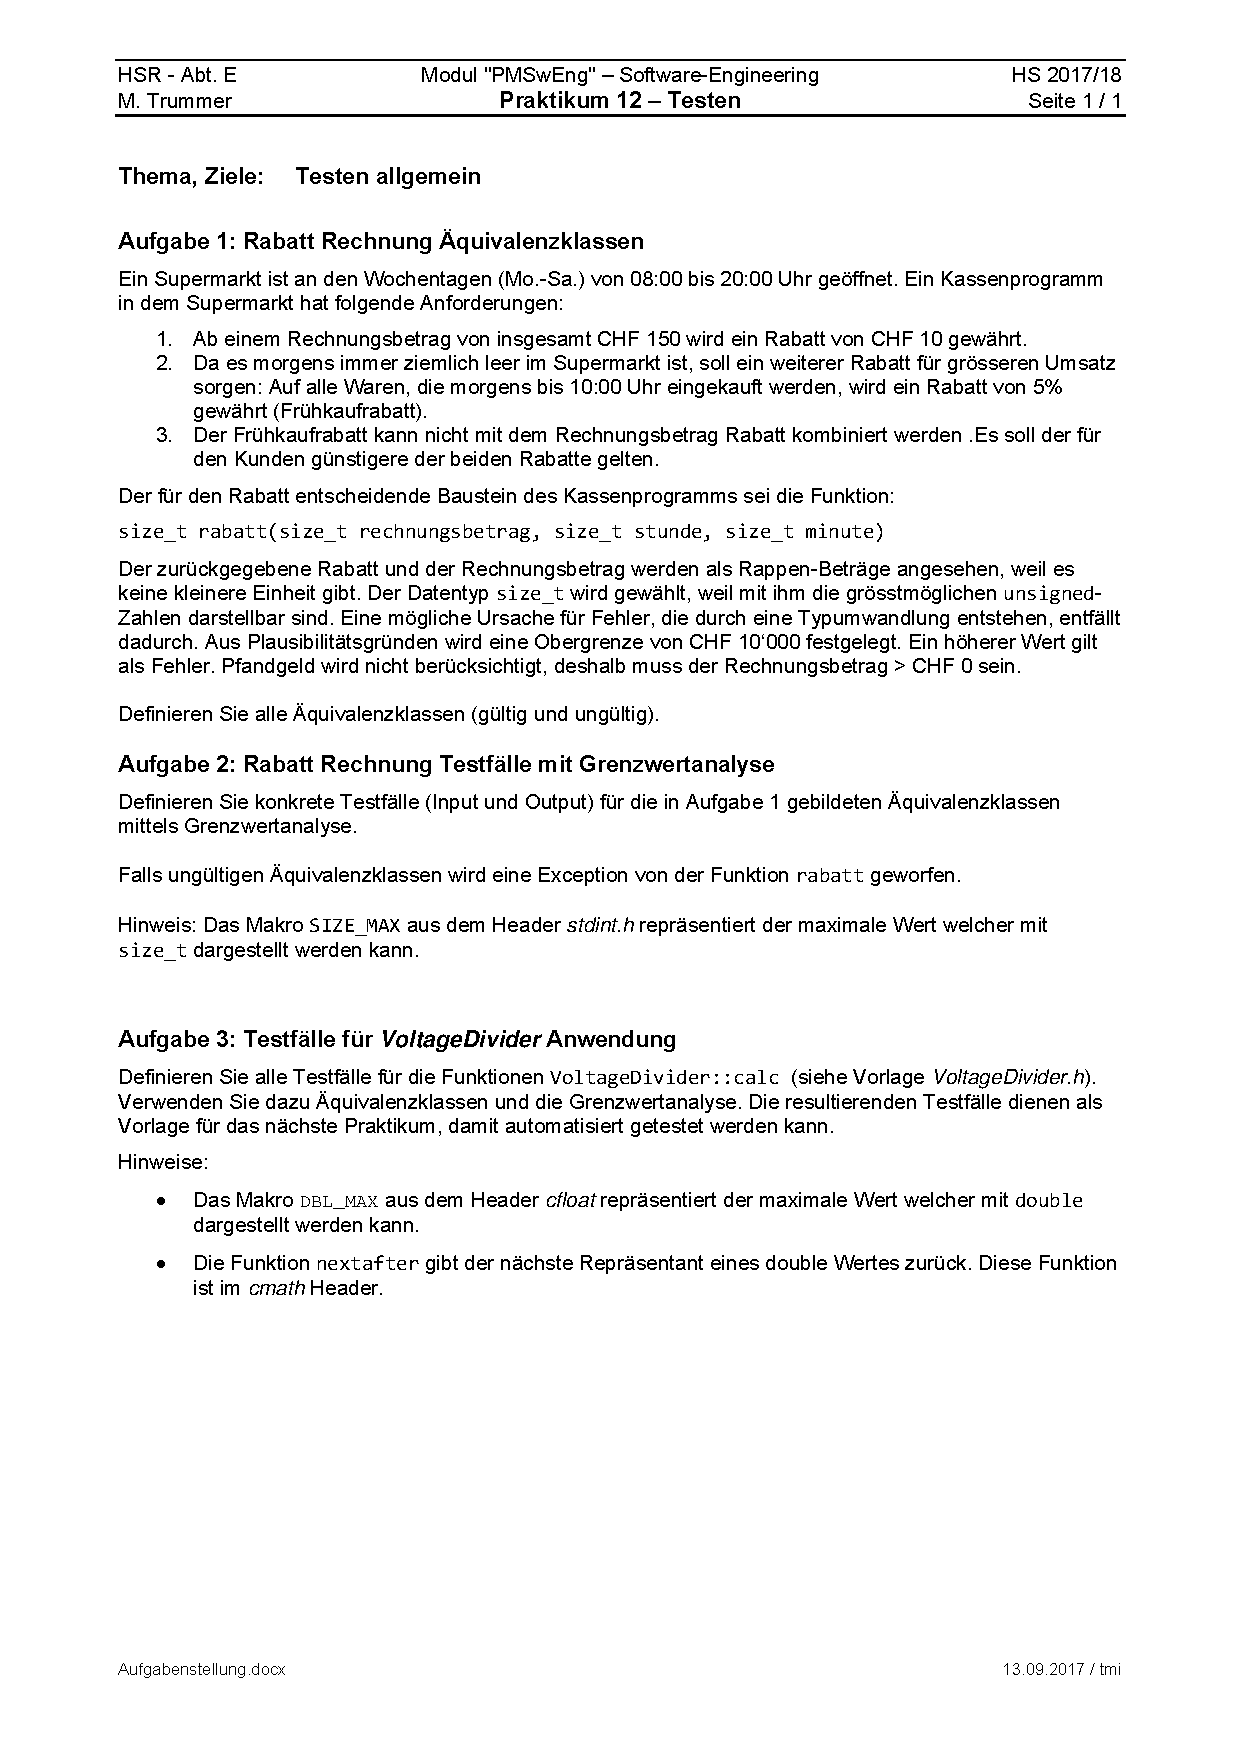
\includepdf[pages=-]{./Uebungen/prak12/Aufgabenstellung.pdf}
%\includepdf[pages=-]{./Uebungen/prak12/Loesung.pdf}
%
%%Uebung 13
%\setcounter{section}{13}
%\setcounter{subsection}{1}
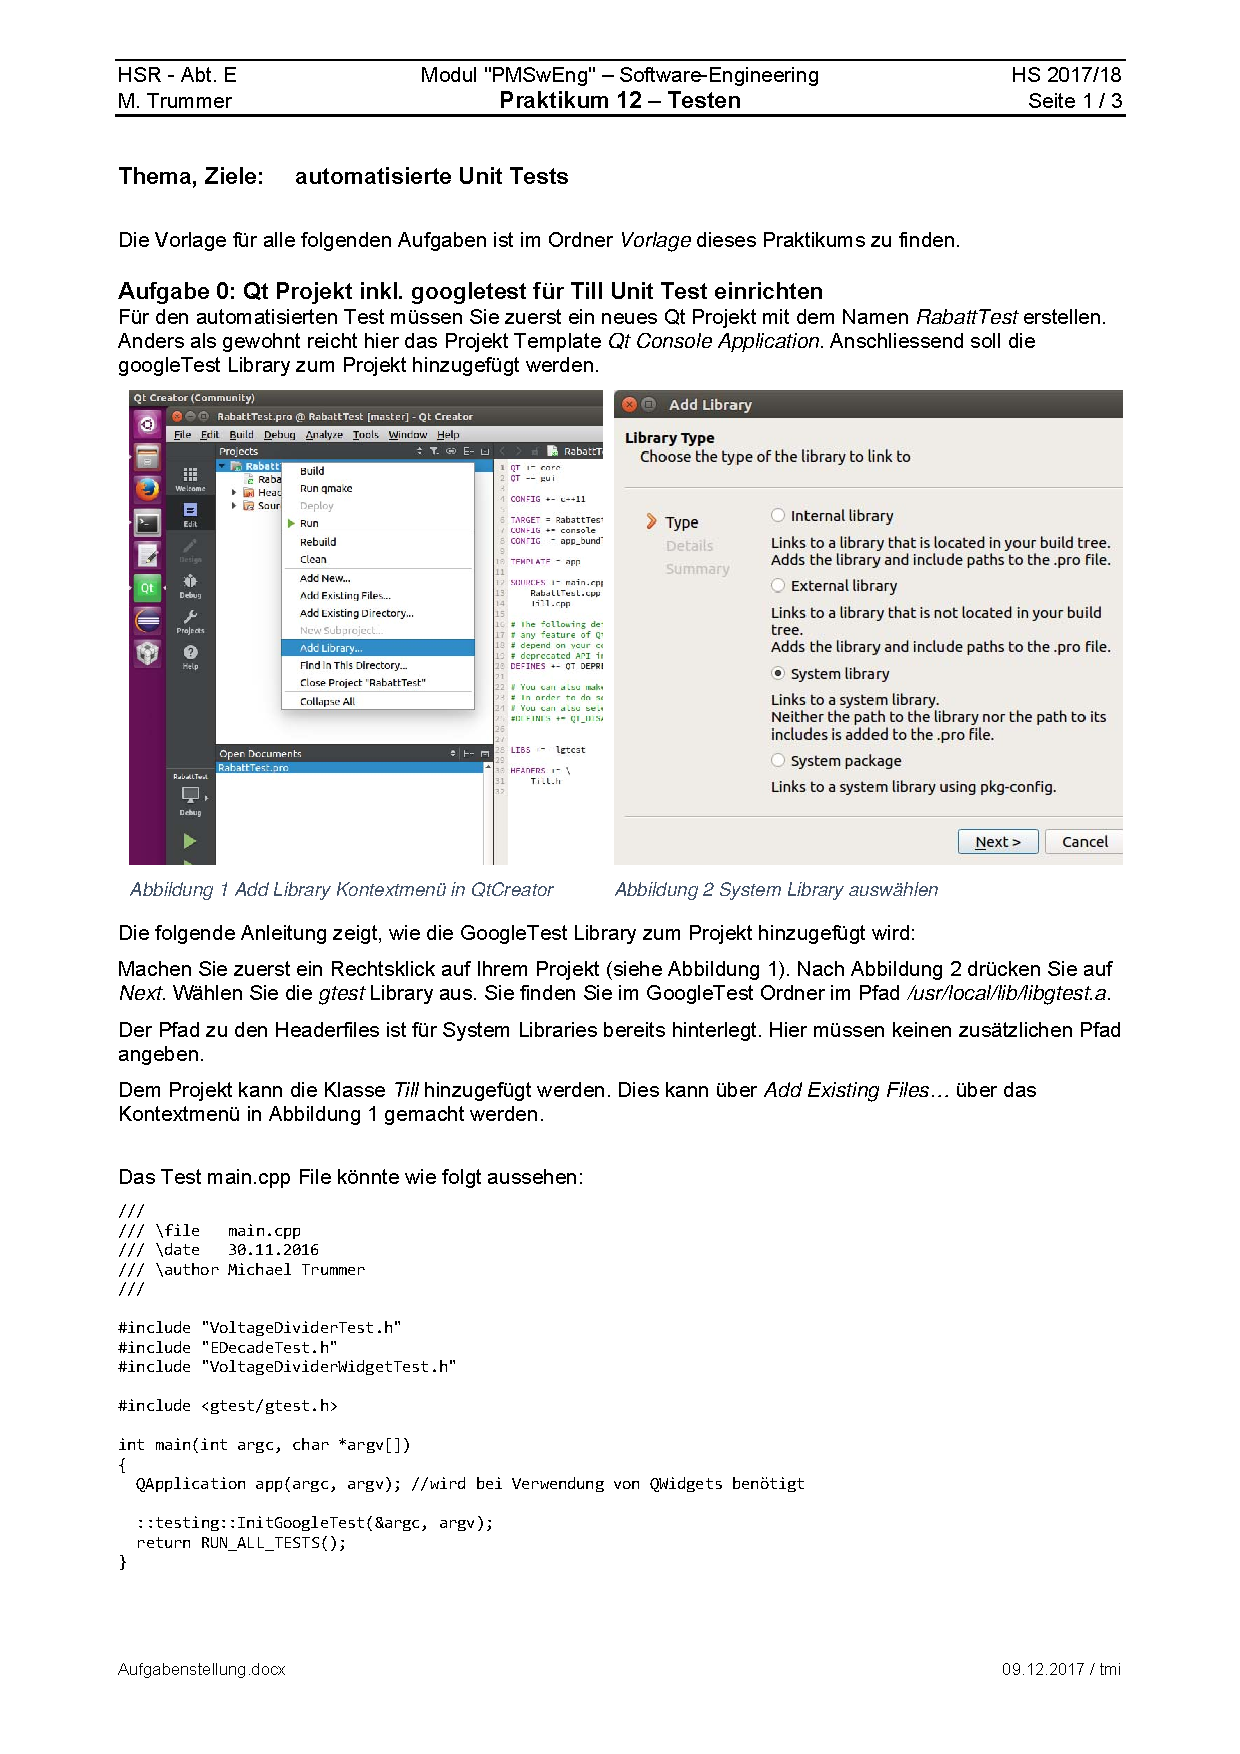
\includepdf[pages=-]{./Uebungen/prak13/Aufgabenstellung.pdf}
%\includepdf[pages=-]{./Uebungen/prak13/Loesung.pdf}
%
%%Uebung 14
%\setcounter{section}{14}
%\setcounter{subsection}{1}
%\includepdf[pages=-]{./Uebungen/prak14/Aufgabenstellung.pdf}
%\includepdf[pages=-]{./Uebungen/prak14/Loesung.pdf}